\section{Limitations}
% 中文：局限性

The signature is English and corpus-conditioned. Fixed-token transport is tested in two models, while selective free-generation evidence is limited to the Llama lexical axis at one development-selected, single-layer 10\% strength. The result is not a universal authorship factor, does not extend automatically to syntax or Qwen generation, and does not establish semantic or perceptual equivalence.
% 中文：该特征基于英文且依赖于语料。固定 token 传输在两个模型中测试，而选择性自由生成证据只针对 Llama 词汇轴以及一个由开发集选择的单层 10\% 强度。该结果不是普适的作者身份因子，不能自动扩展到句法或 Qwen 生成，也不能建立语义或感知等价性。

\section{Ethical Considerations}
% 中文：伦理考虑

The directions are corpus contrasts, not authorship detectors. Using them to label writers may disadvantage non-native, neurodivergent, formal, or technical prose and should not support accusations or penalties. The release contains no detector or decision threshold; any use requires human review and an appeal route.
% 中文：这些方向是语料对比，而不是作者身份检测器。用它们标记作者可能会对非母语、神经多样性、正式或技术文本造成不利影响，因此不应据此提出指控或实施惩罚。发布内容不包含检测器或决策阈值；任何使用都需要人工审查和申诉渠道。

\section{Corpus and Surface Evidence}
\label{app:moved-overview}
\label{app:method-detail}
% 中文：语料与表面证据

This section expands the corpus, measurement, and surface-transfer stages summarized above. All numerical panels are generated from frozen observation files.
% 中文：本节展开上文概述的语料、测量与表面迁移阶段。所有数值图均由冻结的观测文件生成。

\subsection{Estimands}
% 中文：估计目标

Table~\ref{tab:estimands-at-glance} separates the evaluation units used at each stage; the following material supplies the complete construction and evaluation details for those estimands.
% 中文：表~\ref{tab:estimands-at-glance} 区分了各阶段的评估单位；以下内容给出这些估计目标的完整构造与评估细节。

\begin{figure*}[!t]
\centering
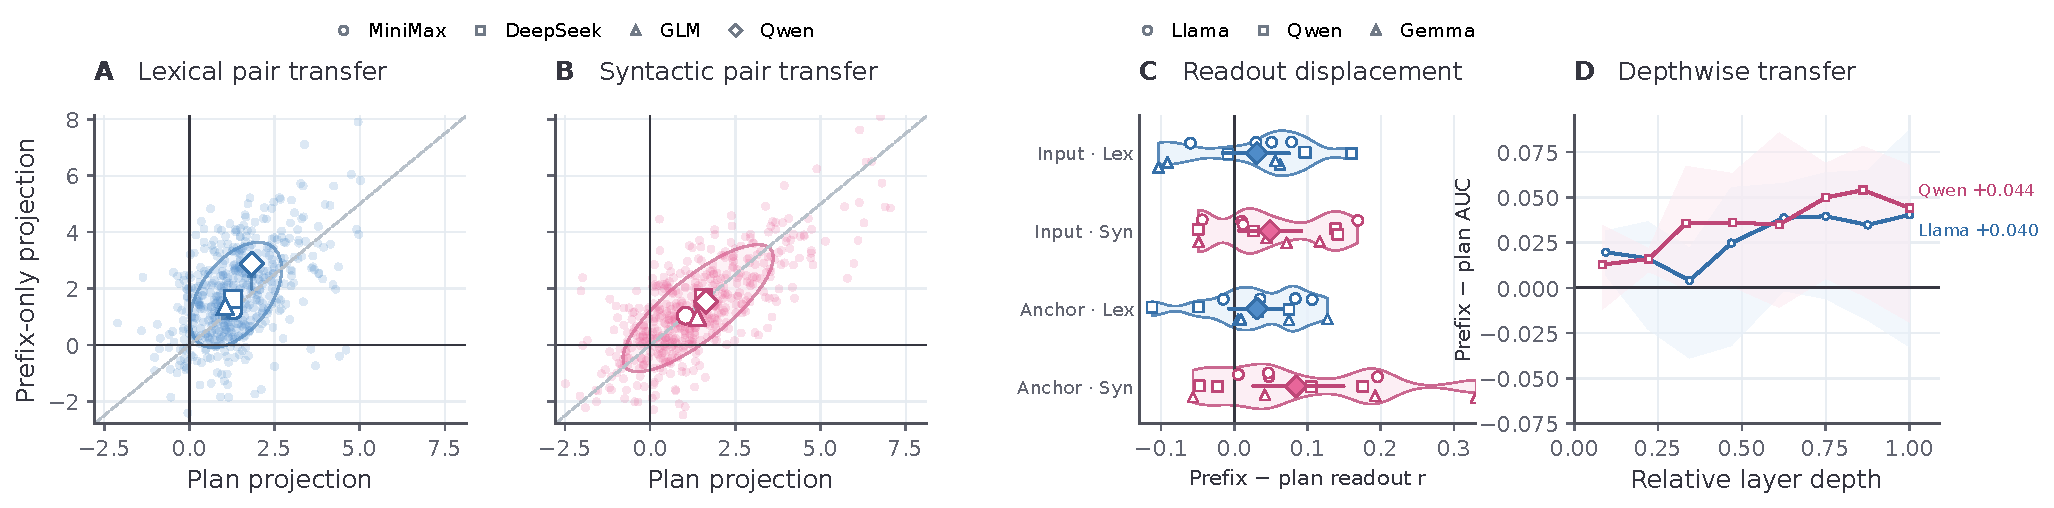
\includegraphics[width=\textwidth]{figures/appendix_surface_transfer.pdf}
\caption{\textbf{Surface directions transfer after removing the proposition plan.} (A--B) Pair projections. (C) Readout-correlation changes at input and anchor layers. (D) Source-separation changes across depth. Prefix-only data are held out from fitting.}
% 中文图注：移除命题计划后，表面方向仍然能够迁移。(A--B) 样本对投影；(C) 输入层和锚点层的读出相关变化；(D) 随深度变化的来源分离。纯前缀数据不参与拟合。
\label{fig:app-surface-transfer}
\end{figure*}

\subsection{Corpus and Measures}
\label{app:corpus-detail}
% 中文：语料与测量

\paragraph{Proposition-conditioned corpus.} Human continuations are balanced across PG-19 narrative, WikiLingua instructional text, Wikipedia encyclopedic text, and XL-Sum news, with 125 pairs from each source. Generation is balanced across MiniMax-M2.5, DeepSeek-V4-Flash, GLM-5.2, and Qwen3.6-Flash. A planner sees the natural prefix and human continuation and records 3--10 atomic propositions, required entities, and an intended endpoint. A distinct generator sees the prefix and plan but never the human continuation, and planner, generator, and judge are distinct for every pair. Acceptance requires complete or mostly complete core-content coverage, no major unsupported claim, and no major contradiction. Structural gates reject malformed, list-like, meta, refused, excessively copied, or extreme-length candidates; rejected attempts are regenerated, not edited. The resulting pairs are proposition-conditioned automatically, while semantic and rhetorical equivalence remains an empirical diagnostic.
% 中文：\textbf{命题条件分支。} 人类续写在 PG-19 叙事文本、WikiLingua 指导文本、Wikipedia 百科文本和 XL-Sum 新闻文本之间保持平衡，每个来源包含 125 对样本；生成任务也在 MiniMax-M2.5、DeepSeek-V4-Flash、GLM-5.2 与 Qwen3.6-Flash 之间保持平衡。规划器读取自然前缀与人类续写，并记录 3--10 个原子命题、必需实体和预期终点。另一个独立生成器读取前缀与计划，但从不读取人类续写；每一对样本的规划器、生成器和评审器均彼此不同。样本被接受的条件是核心内容得到完整或基本完整的覆盖，不包含重大的无依据主张，也不存在重大矛盾。结构门控会拒绝格式异常、列表化、元话语、拒答、过度复制或长度极端的候选文本；被拒绝的候选会重新生成，而不会被编辑修补。由此得到的样本对由自动流程施加命题条件，而语义与修辞等价性仍作为经验诊断加以检验。

\paragraph{Prefix-only corpus.} For each accepted sample, the control retains its identifier, source, natural prefix, human continuation, assigned generator, and target word count. The generator receives only the prefix and scalar length request---never the plan, entity list, endpoint, human continuation, or a transformation of them. It passes the same structural gates but no content-overlap gate. This arm removes the asymmetric planning interface and has weaker semantic matching. Axes and readouts evaluated on this arm are fitted exclusively on the proposition-conditioned corpus.
% 中文：\textbf{仅前缀分支。} 对每个已接受样本，控制分支保留其标识符、来源、自然前缀、人类续写、指定生成器和目标词数。生成器只接收前缀和标量长度要求，绝不会接收计划、实体列表、终点、人类续写或它们的任何变换。该分支通过相同的结构门控，但不使用内容重合门控。它移除了不对称的规划接口，但语义匹配更弱。在该分支上评估的轴和读出均只使用命题条件语料进行拟合。

\paragraph{Corpus ledger.} The proposition-conditioned corpus contains 500 accepted pairs, balanced at 125 per domain and generator. All 500 pass the independent automatic judge and maintain distinct planner, generator, and judge models. The construction log records 50 rejected generations, including 43 rejected candidate records; accepted texts receive no post-generation repairs. The non-gating plan-serialization diagnostic flags 179 pairs, but the extreme serialization gate flags none. Mean and median machine--human length ratios are 0.935 and 0.925, with range 0.603--1.405. The proposition-conditioned semantic cosine is 0.925, the prefix-only cosine is 0.727, and within-source derangement gives 0.469. These records support controlled comparison but do not certify perfect propositional equivalence.
% 中文：\textbf{语料账本。} 命题条件语料包含 500 对已接受样本，并在领域和生成器两个维度上各自保持每组 125 对的平衡。全部 500 对均通过独立自动评审，且每对样本的规划器、生成器与评审器模型彼此不同。构建日志记录了 50 次被拒绝的生成，其中包括 43 条被拒绝的候选记录；已接受文本不进行生成后的修补。非门控的计划序列化诊断标记了 179 对样本，而极端序列化门控未标记任何样本。机器文本与人类文本长度比的均值和中位数分别为 0.935 和 0.925，范围为 0.603--1.405。命题条件分支的语义余弦为 0.925，仅前缀分支为 0.727，而同来源错配基线为 0.469。这些记录支持受控比较，但并不证明命题完全等价。

\paragraph{Measurement.} The frozen inventory contains 10 lexical, 12 syntactic, and 13 discourse measurements. Seven nuisance variables---word, sentence, paragraph, and character counts, mean sentence length, named-entity rate, and number rate---are removed by training-fold regression. Feature standardization, nuisance fitting, surface-axis construction, and hidden readout fitting all occur inside the relevant training fold. The discourse group remains an off-target audit rather than a stable hidden target. Section~\ref{app:features} gives the dictionary, strongest effects, complete environment holdouts, plan-removal control, and PCA sensitivity.
% 中文：\textbf{测量与拟合。} 冻结的指标库包含 10 个词汇指标、12 个句法指标和 13 个篇章指标。七个干扰变量通过训练折内回归移除，包括词数、句数、段落数、字符数、平均句长、命名实体比例和数字比例。特征标准化、干扰项拟合、表层轴构建和隐藏读出拟合均在相应训练折内部完成。篇章指标组仅作为非目标审计，而不是稳定的隐藏目标。第~\ref{app:features} 节给出完整指标字典、最强效应、全部环境留出结果、移除计划的控制实验和 PCA 敏感性分析。

\paragraph{Feature inventory.} The 10 lexical coordinates are function-word, pronoun, contraction, repeated-trigram, abstract, evaluative, emphasis, and institutional-lexicon rates, MATTR-50, and mean content-word Zipf frequency. The 12 syntactic coordinates are mean dependency depth and length; clause, coordination, and subordination densities; passive-clause, nominalization, fragment, apposition, and parenthetical rates; sentence-length coefficient of variation; and adjacent POS parallelism. The 13 discourse coordinates cover six connective families, explicit relations, transition openings, enumeration and summary markers, entity and subject continuity, and adjacent content overlap. Lexical and syntactic groups are hidden-state targets; discourse is an off-target audit. Every training fold residualizes word, sentence, paragraph, and character counts, mean sentence length, named-entity rate, and number rate.
% 中文：\textbf{冻结指标字典。} 10 个词汇坐标包括功能词、代词、缩略形式、重复三元组、抽象词、评价词、强调词和机构词汇的比例，以及 MATTR-50 和实义词平均 Zipf 频率。12 个句法坐标包括平均依存深度与长度，分句、并列和从属结构密度，被动分句、名词化、句子片段、同位结构和插入结构比例，句长变异系数，以及相邻词性序列平行度。13 个篇章坐标覆盖六类连接词、显式关系、过渡性开头、列举和总结标记、实体与主语连续性，以及相邻内容重合度。词汇组和句法组是隐藏状态目标，篇章组用于非目标审计。每个训练折都会对词数、句数、段落数、字符数、平均句长、命名实体比例和数字比例进行残差化处理。

\subsection{Surface Realizations}
\label{app:features}
% 中文：表面实现

\paragraph{Linguistic interpretation.} The multivariate projection corresponds to recurrent, readable choices. Across 500 matched pairs, \emph{however} appears in 83 machine documents and 34 human documents; \emph{these} in 116 and 69; \emph{during} in 78 and 49; \emph{despite} in 36 and 7; and \emph{following} in 35 and 14. Evaluative forms also separate the sources: \emph{crucial} and \emph{significant} each occur in 22 machine documents but only 3 human documents. The reporting frames \emph{stated that} and \emph{noted that} likewise occur in 16 and 13 machine documents and in no matched human document. These counts describe this corpus; none is an authorship criterion.
% 中文：\textbf{这些样本对中的“类 AI”含义。} 多变量投影对应反复出现且可直接辨认的语言选择。在 500 对匹配样本中，\emph{however} 出现在 83 篇机器文档和 34 篇人类文档中；\emph{these} 分别为 116 和 69 篇；\emph{during} 为 78 和 49 篇；\emph{despite} 为 36 和 7 篇；\emph{following} 为 35 和 14 篇。评价性形式也区分了两个来源：\emph{crucial} 和 \emph{significant} 各自出现在 22 篇机器文档中，但在人类文档中都只有 3 篇。报道框架 \emph{stated that} 和 \emph{noted that} 分别出现在 16 和 13 篇机器文档中，而在匹配的人类文档中均未出现。这些计数只描述本语料，任何单项都不是作者身份判据。

\paragraph{Distributed effects.} The largest standardized shifts span both confirmatory groups: function-word rate decreases by \(d=-1.221\), pronoun rate by \(-0.770\), and mean content-word frequency by \(-0.759\); lexical diversity increases by \(+0.659\), while mean dependency length and sentence-length variation decrease by \(-0.654\) and \(-0.491\). Their distribution across measurements motivates a multivariate signature rather than a single-cue detector.
% 中文：\textbf{分布式特征效应。} 最大的标准化位移跨越两个验证性指标组：功能词比例下降 \(d=-1.221\)，代词比例下降 \(-0.770\)，实义词平均频率下降 \(-0.759\)；词汇多样性增加 \(+0.659\)，平均依存距离与句长变异分别下降 \(-0.654\) 和 \(-0.491\)。这些变化分布在多个测量上，因此本文采用多变量特征，而不是单线索检测器。

\paragraph{Paired evidence.} The same tendency appears as rhetorical repackaging within proposition-conditioned pairs. A human news continuation begins, ``In a statement, RBS chief executive Ross McEwen said \ldots,'' whereas its machine mate writes, ``RBS chief executive Ross McEwen stated that \ldots.'' A human narrative coordinates survival with ``Yet he stood on his feet,'' while the machine makes the relation explicit: ``Despite this grievous injury, he pressed on.'' An instructional sentence changes from ``You should consider if the beginning section flows well'' to ``It is crucial to check whether the beginning flows naturally.'' The examples instantiate the measured shifts toward explicit transitions, nominal or evaluative framing, and more regular clause packaging. They are concordances for interpreting the frozen measurements.
% 中文：\textbf{句子级配对证据。} 同一趋势在命题条件样本对中表现为修辞重组。一段人类新闻续写以“In a statement, RBS chief executive Ross McEwen said \ldots”开头，而其机器配对文本写作“RBS chief executive Ross McEwen stated that \ldots”。一段人类叙事用“Yet he stood on his feet”连接生还情节，机器文本则用“Despite this grievous injury, he pressed on”显式表达这一关系。一个指导性句子从“You should consider if the beginning section flows well”变为“It is crucial to check whether the beginning flows naturally”。这些例子具体呈现了测量到的变化，即更显式的过渡、更强的名词性或评价性框架，以及更规则的分句组织。它们用于帮助解释冻结指标，而不参与指标拟合。

Figure~\ref{fig:app-surface-transfer} separates pair-level transfer from hidden readout transfer. Most continuations remain in the machineward quadrant at both interfaces, while the paired scatter exposes which samples move toward or across the decision origin. Across the input-to-anchor displacements, proposition-conditioned and prefix-only readout correlations are related but not interchangeable. The depth profiles show that removing the plan usually improves source separation while retaining visible generator variation.
% 中文：图~\ref{fig:app-surface-transfer} 将样本对层面的迁移与隐藏读出的迁移区分开来。多数续写在两个接口下都位于机器方向象限，而配对散点揭示了哪些样本向决策原点移动或越过原点。从输入层到锚点的位移表明，命题条件读出与仅前缀读出彼此相关，但不能互换。深度剖面显示，移除计划通常会提高来源分离度，同时保留可见的生成器差异。

Lexical and syntactic directions remain stable under generator holdout. Their domain-minimum cosines are lower, at 0.934 and 0.546, but remain positive. On prefix-only outputs, the original-axis lexical and syntactic cosines are 0.885 and 0.869, with positive projections for 88.0\% and 79.6\% of pairs. The discourse direction collapses in its weakest environments and under aggressive PCA truncation and remains an off-target measurement. On the prefix-only corpus, lexical and syntactic readouts remain predictive even though the generator receives no human-derived proposition plan.
% 中文：词汇方向和句法方向在生成器留出条件下保持稳定。它们在领域留出下的最小余弦较低，分别为 0.934 和 0.546，但仍为正值。在纯前缀输出上，原始轴的词汇和句法余弦分别为 0.885 和 0.869，且分别有 88.0\% 和 79.6\% 的样本投影为正。篇章方向在最弱环境和激进 PCA 截断下发生坍缩，因此仍只作为非目标测量。在仅前缀语料上，尽管生成器没有接收任何源自人类文本的命题计划，词汇与句法读出仍具有预测性。

\begin{figure*}[!t]
\centering
\begin{tcbraster}[raster columns=2,raster equal height=rows,raster column skip=6pt,raster row skip=5pt]
\begin{tcolorbox}[evidencecard,title={\textbf{A}\quad\textsc{How-to}\hfill\textit{Advice \(\rightarrow\) prescription}}]
\fontsize{7.2}{8.4}\selectfont
\evidrow{\evidhuman}{\textquotedblleft Consider getting it professionally cleaned rather than doing it yourself.\textquotedblright}\par\vspace{2pt}
\evidrow{\evidmachine}{\textquotedblleft Due to their delicate nature, professionally cleaned viscose rugs are strongly recommended over DIY cleaning methods.\textquotedblright}
% 中文：A，指导文本将个人建议改写为一般性的强烈建议。
\end{tcolorbox}
\begin{tcolorbox}[evidencecard,title={\textbf{B}\quad\textsc{News}\hfill\textit{Attribution \(\rightarrow\) argument}}]
\fontsize{7.2}{8.4}\selectfont
\evidrow{\evidhuman}{She said A\&E services had been ``ground down so much'' that something less can be classed as a major incident.}\par\vspace{2pt}
\evidrow{\evidmachine}{However, she argued that A\&E services have degraded to such an extent that lesser events now qualify.}
% 中文：B，新闻文本将一般报道动词改写为论证性更强、关系更显式的表达。
\end{tcolorbox}
\begin{tcolorbox}[evidencecard,title={\textbf{C}\quad\textsc{Biography}\hfill\textit{Sequence \(\rightarrow\) transition}}]
\fontsize{7.2}{8.4}\selectfont
\evidrow{\evidhuman}{After cutting short his stay with Terengganu FA, Faiz signed a contract with Penang FA along with teammate Mazlizam Mohamad.}\par\vspace{2pt}
\evidrow{\evidmachine}{Subsequently, Faiz signed with Penang FA alongside Terengganu FA teammate Mazlizam Mohamad.}
% 中文：C，百科文本将叙事性顺序改写为带有显式阶段标记的过渡。
\end{tcolorbox}
\begin{tcolorbox}[evidencecard,title={\textbf{D}\quad\textsc{Literary}\hfill\textit{Question \(\rightarrow\) causality}}]
\fontsize{7.2}{8.4}\selectfont
\evidrow{\evidhuman}{\textquotedblleft Why prematurely claim to have reached finality, when unexpected novelties may shatter any system before it is even completed?\textquotedblright}\par\vspace{2pt}
\evidrow{\evidmachine}{\textquotedblleft Claiming finality is premature because unexpected novelties can shatter any system before completion.\textquotedblright}
% 中文：D，文学文本将完整的修辞问句改写为使用 because 明示关系的陈述性因果表达。
\end{tcolorbox}
\end{tcbraster}
\caption{\textbf{Rhetorical repackaging across domains.} Complete paired excerpts illustrate prescription, argument, explicit transition, and causality; none enters model fitting.}
% 中文图注：跨领域的修辞重组。完整配对摘录分别展示处方式建议、论证性表达、显式过渡和明确因果；所有摘录均不参与模型拟合。
\label{fig:realization-examples}
\end{figure*}

\subsection{Lexical Concordance}
% 中文：词汇一致性
\label{app:concordance}

\paragraph{Lexical inventory.} The more conspicuous connective choices sharpen the corpus-level description: \emph{consequently} occurs in 21 machine documents and 1 human document, \emph{furthermore} in 11 and 1, \emph{additionally} in 15 and 5, and \emph{ultimately} in 11 and 1. Evaluative closure shows the same asymmetry: \emph{essential} occurs in 16 machine documents and 2 human documents, and \emph{profound} in 7 and 0. The full frame \emph{it is crucial} occurs in 10 machine continuations and no human continuation.
% 中文：\textbf{连接词与评价词清单。} 更显眼的连接词选择进一步明确了语料层面的特征：\emph{consequently} 出现在 21 篇机器文档和 1 篇人类文档中，\emph{furthermore} 为 11 和 1 篇，\emph{additionally} 为 15 和 5 篇，\emph{ultimately} 为 11 和 1 篇。评价性结尾也呈现相同的不对称：\emph{essential} 出现在 16 篇机器文档和 2 篇人类文档中，\emph{profound} 为 7 和 0 篇。完整框架 \emph{it is crucial} 出现在 10 段机器续写中，而未出现在任何人类续写中。

\paragraph{Corpus specificity.} Popular shibboleths do not necessarily separate a matched corpus: \emph{delve} occurs in neither source, \emph{tapestry} occurs once in each, and \emph{landscape} occurs in 6 machine versus 5 human documents. The recognizable contrast lies in the combination of explicit linking, evaluative closure, and regularized clause packaging.
% 中文：\textbf{语料特异性。} 流行的刻板线索未必能够区分匹配语料：\emph{delve} 在两个来源中都未出现，\emph{tapestry} 在两侧各出现一次，\emph{landscape} 则出现在 6 篇机器文档和 5 篇人类文档中。可辨认的差异来自显式连接、评价性收束和规则化分句组织的组合。
\paragraph{Paired excerpts.} The four readings below show how corpus-level effects appear in individual pairs. Instructions move from personal advice to impersonal prescription; news replaces repeated \emph{said} with differentiated reporting predicates; encyclopedic prose adds explicit stage and evaluation markers; and literary rhetorical questions become declarative causal relations. Across domains, the recurring pattern is rhetorical regularization.
% 中文：\textbf{补充配对摘录。} 下面四组文本展示语料层面的效应如何出现在具体样本对中。指导文本从个人建议转向非人称规范；新闻文本用功能区分更细的报道谓词替代重复的 \emph{said}；百科文本加入显式的阶段与评价标记；文学文本中的修辞问句转化为陈述性的因果关系。跨领域反复出现的模式是修辞表达的规则化。

\paragraph{Same-token field.}\label{app:token-field} We also project 2.44--2.48M continuation-token states per model onto leave-one-generator-out nuisance-nullspace directions. An exact token is compared only in matched pairs containing it on both sides, after subtracting each continuation's mean coordinate; source separation and unequal frequency are removed from the local contrast. Of 612--704 eligible contrasts per model, 89--379 survive BH-FDR and generator/domain sign-agreement gates. The field is specific to each model and tokenizer and is estimated from hidden-state projections rather than direct-logit-lens decoding.
% 中文：\textbf{投影限定的词汇场。} 我们还将每个模型的 244 万至 248 万个续写 token 状态投影到留一生成器的干扰零空间方向上。只有当某个精确 token 同时出现在匹配样本对两侧时才进行比较，并先减去各自续写的平均坐标；这种局部对比移除了来源分离和频率不等的影响。每个模型有 612--704 个合格对比，其中 89--379 个通过 BH-FDR 以及生成器与领域符号一致性门控。该词汇场由模型和分词器共同决定，并通过隐藏状态投影估计，而不是通过直接的 logit-lens 解码获得。
% The hidden-state block is compiled from main_hidden_details.tex at its corresponding location in the main method.

\section{Readout and Pullback}
\label{app:direction-detail}
% 中文：读出与回拉

\paragraph{Readout.} For source side \(a\), let \(H_a\) be centered, nuisance-residualized hidden states in the frozen within-class nullspace and \(z_{ga}\) the corresponding centered surface scores. Equation~\ref{eq:covariance-readout} defines the forward covariance activation pattern and the source-consensus readout. Human and machine patterns must agree positively before their normalized sum. The reported fold statistic averages the two held-out Pearson correlations; Table~\ref{tab:readout-folds} retains both source-side values.
% 中文：\textbf{读出。} 对来源侧 \(a\)，令 \(H_a\) 表示在冻结的类内干扰零空间中经过中心化与干扰残差化的隐藏状态，令 \(z_{ga}\) 表示对应的中心化表层分数。公式~\ref{eq:covariance-readout} 定义了前向协方差激活模式与来源共识读出。人类侧与机器侧模式必须具有正向一致性，随后才对其归一化求和。报告的折级统计量对两个留出来源侧的 Pearson 相关取平均；表~\ref{tab:readout-folds} 保留两个来源侧的数值。




\paragraph{Pullback.} Equation~\ref{eq:pullback-main} maps each late readout through the layer-to-layer Jacobian, averages source-side pullbacks, and projects them through the frozen nuisance projector \(P_m\). Neither source-side vector is sign-flipped, so the declared \(+w\) pole is inherited from the machine-oriented readout. Equation~\ref{eq:transport-response} defines the fixed-sequence response: signed \(\tau\) gives directionality, while \(|\tau|\) gives capacity comparable with unoriented null targets.
% 中文：\textbf{回拉与带符号响应。} 公式~\ref{eq:pullback-main} 通过层间 Jacobian 映射每个后期读出器，对来源侧回拉取平均，并通过冻结的干扰投影器 \(P_m\) 进行投影。两个来源侧向量都不会翻转符号，因此预先声明的 \(+w\) 极点继承自机器方向读出器。公式~\ref{eq:transport-response} 定义固定序列响应：带符号的 \(\tau\) 表示方向性，\(|\tau|\) 表示可与无语义方向零目标比较的传输容量。

\paragraph{Matched null.} Each replicate permutes surface scores within corpus--generator strata, refits every layerwise readout, refreezes the global direction, repeats the Jacobian pullback, and evaluates the identical hashed trajectories. The learned and refitted-null capacities are defined in Equation~\ref{eq:transport-response}. We use \(n=100\), \(R=100\), five intermediate layers, and a depth-normalized curve statistic. Injection and fitted readout-anchor layers remain descriptive construction-internal diagnostics.
% 中文：\textbf{匹配管线零分布。} 每个重复实验在语料--生成器分层内部置换表层分数，重新拟合每一层读出器，重新冻结全局方向，重复 Jacobian 回拉，并在完全相同的哈希轨迹上评估。学习容量与重拟合零容量在公式~\ref{eq:transport-response} 中定义。实验使用 \(n=100\)、\(R=100\)、五个中间层以及按深度归一化的曲线统计量。注入层和已拟合的读出锚点层只保留为描述性的构建内部诊断。

Figure~\ref{fig:app-hidden-robustness} compares construction alternatives, nuisance ranks, and fit counts for all four model--axis cases.
% 中文：图~\ref{fig:app-hidden-robustness} 比较了四个模型--轴组合中的构建替代方案、干扰秩和拟合样本数。

\begin{figure*}[!t]
    \centering
    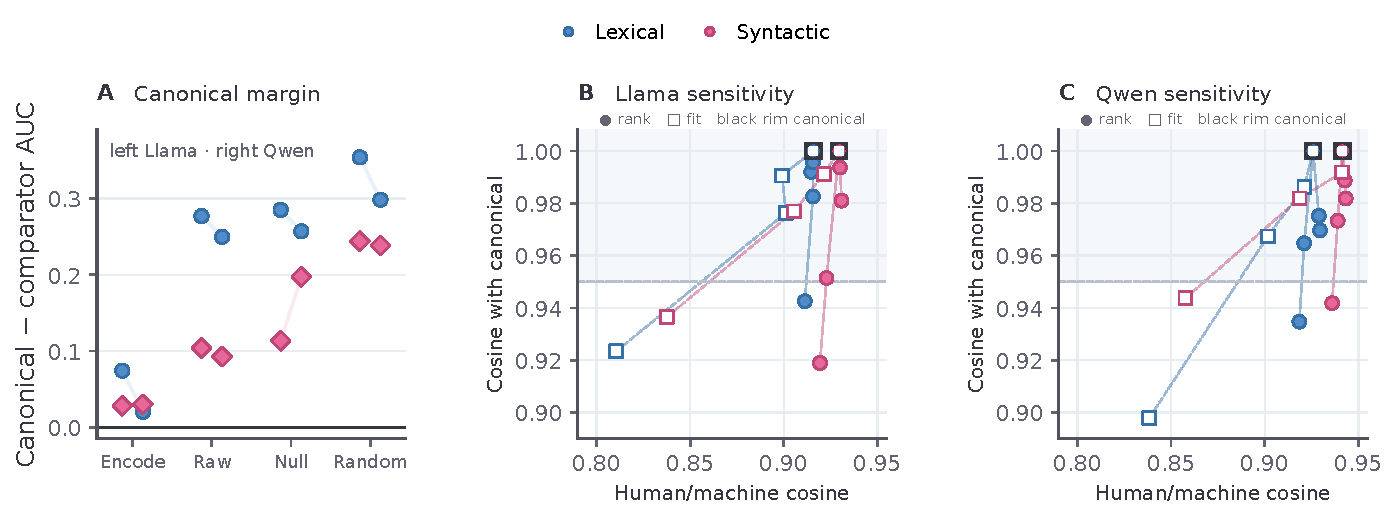
\includegraphics[width=\textwidth]{figures/appendix_hidden_robustness.pdf}
\caption{\textbf{Canonical pullback is stable across construction choices.} (A) Capacity margin over four alternatives. (B--C) Nuisance-rank and fit-size variants; black rings mark the frozen setting.}
% 中文图注：规范回拉在不同构造选择下保持稳定。(A) 相对四种替代方向的容量优势；(B--C) 干扰秩与拟合规模变体，黑色外环标记冻结设置。
\label{fig:app-hidden-robustness}
\end{figure*}

The canonical pullback exceeds upstream encoding, raw source contrast, nullspace source contrast, and the projected-random ensemble in all four model--axis cases. The margin over upstream encoding is smaller than the margins over the other controls, consistent with related but distinct encoding and pullback geometry. All nuisance-rank and fit-count variants remain close to the frozen direction. Figure~\ref{fig:hidden-trace} contains the fixed-token trajectories and matched-null distributions.
% 中文：在四个模型--轴组合中，规范回拉均超过上游编码、原始来源对比、零空间来源对比和投影随机集合。相较于上游编码的优势小于相较于其他控制方向的优势，这与编码几何和回拉几何相关但不同的解释一致。所有干扰秩和拟合样本数变体都接近冻结方向。图~\ref{fig:hidden-trace} 给出固定 token 轨迹和匹配零分布。

\section{Generation Evidence}
% 中文：生成证据

This section separates the held-out lexical test from the earlier low-dose audit and records the inference and artifact boundary.
% 中文：本节将持出词汇检验与较早的低剂量审计分开，并记录推断与实验制品边界。

\subsection{Held-Out Lexical Test}
\label{app:seed-detail}
% 中文：持出词汇检验

\paragraph{Protocol.} Hooks begin after prompt prefill. The canonical Llama lexical pullback is injected at L7 with mean pooling, and \(+w\) retains the machine-oriented pole fixed by the readout. Prompt indices 0--19 form a development set used to select \(\alpha=2\), or 10\% of the mean hidden-state norm. After this choice, the intervention site, pole, strength, 128-new-token budget, temperature 0.7, top-\(p=0.95\), and base seed 8236 are frozen. The formal test uses the untouched prompt indices 34--199, giving 166 prompts and three paired decode seeds.
% 中文：协议。Hook 在提示预填充后启动。规范的 Llama 词汇回拉以均值池化方式注入 L7，\(+w\) 保留由读出器预先固定的机器方向极性。索引 0--19 的提示构成开发集，用于选择 \(\alpha=2\)，即平均隐藏状态范数的 10\%。完成选择后，干预位置、极性、强度、128 个新 token 的预算、温度 0.7、top-\(p=0.95\) 和基础随机种子 8236 全部冻结。正式检验使用未参与调参的索引 34--199，共 166 个提示和三个配对解码种子。

\paragraph{Inference.} The prompt is the unit of inference. We compute the paired \(+2w/-2w\) difference within each seed, average the three differences within prompt, and bootstrap the 166 prompt means. Target projection, aggregate component selectivity, and the two target-minus-off-target contrasts use this same hierarchy; sign-flip tests also operate on the paired prompt means. Repeated decoding refines a prompt-level contrast without treating seeds or tokens as independent observations.
% 中文：推断。推断单位是提示。我们先在每个种子内部计算配对的 \(+2w/-2w\) 差值，再在提示内部平均三个差值，并对 166 个提示均值进行 bootstrap。目标投影、总体成分选择性以及两个目标减非目标对比都使用相同层级；符号翻转检验也作用于配对提示均值。重复解码提高提示级对比的精度，但不会把种子或 token 当作独立观测。

\paragraph{Result.} Lexical target projection is \(0.269\,[0.127,0.412]\) with paired \(d=0.280\) and \(p=0.0006\); component selectivity is \(0.287\,[0.117,0.459]\) with \(d=0.255\) and \(p=0.0012\). The target-minus-syntax contrast is \(0.234\,[0.011,0.457]\), and target-minus-discourse is \(0.340\,[0.184,0.496]\). Target and selectivity seed means are respectively 0.123/0.267/0.416 and 0.090/0.300/0.471, so both estimands retain the declared sign in every seed.
% 中文：结果。词汇目标投影为 \(0.269\,[0.127,0.412]\)，配对 \(d=0.280\)、\(p=0.0006\)；成分选择性为 \(0.287\,[0.117,0.459]\)，\(d=0.255\)、\(p=0.0012\)。目标减句法对比为 \(0.234\,[0.011,0.457]\)，目标减篇章对比为 \(0.340\,[0.184,0.496]\)。目标与选择性的三个种子均值分别为 0.123/0.267/0.416 和 0.090/0.300/0.471，因此两个估计量在每个种子中都保持预先声明的符号。

\begin{figure*}[!t]
\centering
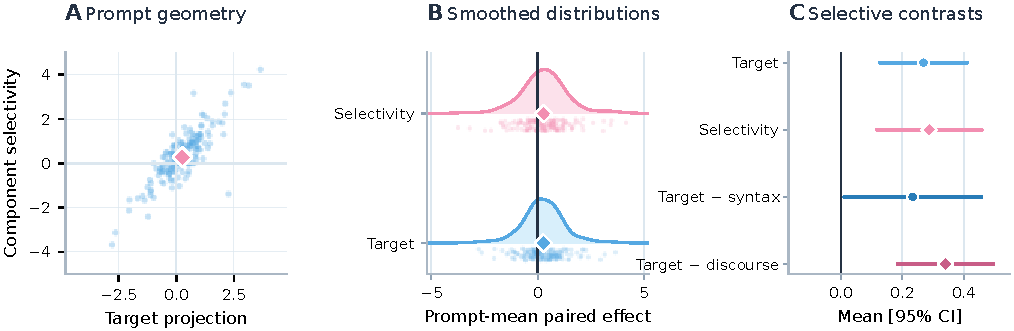
\includegraphics[width=\textwidth]{figures/appendix_generation_robustness.pdf}
\caption{\textbf{Held-out lexical effects across prompts.} (A) Joint prompt geometry. (B) Smoothed marginals. (C) Target and selectivity contrasts with 95\% intervals.}
% 中文图注：提示级持出词汇效应。(A) 提示级联合几何；(B) 平滑边缘分布；(C) 带 95\% 区间的目标与选择性对比。
\label{fig:app-generation-robustness}
\end{figure*}

\paragraph{Prompt variation.} Figure~\ref{fig:app-generation-robustness} retains all 166 prompt coordinates after averaging within prompt across seeds. Target projection and component selectivity are strongly related at the prompt level, while their marginal distributions contain substantial variation on both sides of zero. The positive cluster means and pairwise intervals show that this heterogeneity does not depend on a few seed-level summaries.
% 中文：提示差异。图~\ref{fig:app-generation-robustness} 保留了在提示内部跨种子平均后的全部 166 个提示坐标。目标投影与成分选择性在提示层面高度相关，而二者的边缘分布在零点两侧都存在较大差异。正的聚类均值和成对区间表明，该结果并不依赖少量种子级汇总。

\subsection{Dose Sensitivity}
% 中文：剂量敏感性

Before the held-out test, the 5\% protocol was evaluated across both models and both confirmatory axes. Table~\ref{tab:low-dose-audit} retains those results as a sensitivity analysis. At this lower dose, target movement appears most clearly for Llama syntax, while every component-selectivity interval spans zero. The pattern motivates treating intervention magnitude as a calibrated part of the controller rather than transferring one scale across model--axis conditions.
% 中文：在持出检验之前，5\% 协议曾在两个模型和两个验证性轴上进行评估。表~\ref{tab:low-dose-audit} 将这些结果保留为敏感性分析。在较低剂量下，Llama 句法的目标移动最清晰，但所有成分选择性区间都跨越零。该模式说明，干预强度应被视为需要校准的控制器组成部分，而不能在不同模型—轴组合之间直接沿用同一尺度。

\begin{table}[H]
\centering
\scriptsize
\renewcommand{\arraystretch}{1.05}
\setlength{\tabcolsep}{2.4pt}
\begin{tabular*}{\columnwidth}{@{\extracolsep{\fill}}llrr@{}}
\toprule
\textbf{Model} & \textbf{Axis} & \textbf{Target [95\% CI]} & \textbf{Selectivity [95\% CI]}\\
\midrule
\multirow[c]{2}{*}{Llama 3.1 8B} & Lex. & 0.123 [\textminus0.010, 0.255] & 0.139 [\textminus0.049, 0.345]\\
& Syn. & 0.249 [0.043, 0.518] & 0.152 [\textminus0.092, 0.445]\\
\graymidrule
\multirow[c]{2}{*}{Qwen3 4B} & Lex. & 0.012 [\textminus0.169, 0.195] & 0.027 [\textminus0.181, 0.234]\\
& Syn. & 0.025 [\textminus0.189, 0.295] & 0.029 [\textminus0.221, 0.315]\\
\bottomrule
\end{tabular*}
\caption{\textbf{Low-dose sensitivity.} Prompt-clustered three-seed effects at the 5\% endpoint.}
% 中文表注：低剂量敏感性。5\% 端点上的提示聚类三种子效应。
\label{tab:low-dose-audit}
\end{table}

\paragraph{Guardrails.} The 20-prompt 10\% development run has paired-output semantic similarity \(0.855\,[0.809,0.898]\), with minimum 0.637; its target and selectivity intervals are wide because it is used for selection rather than final inference. Under the broader 5\% audit, paired semantic similarity ranges from 0.864 to 0.875 across the four model--axis conditions, and most content, length, repetition, and fragmentation intervals span zero. These diagnostics support the development choice, but formal 10\% semantic equivalence is not a claim of the held-out experiment.
% 中文：保护指标。20 个提示的 10\% 开发实验中，配对输出语义相似度为 \(0.855\,[0.809,0.898]\)，最小值为 0.637；其目标与选择性区间较宽，因为该数据只用于选择，而不用于最终推断。在更广泛的 5\% 审计中，四个模型—轴条件的配对语义相似度范围为 0.864 到 0.875，并且内容、长度、重复和片段化的大多数区间跨越零。这些诊断支持开发集选择，但持出实验并不据此声称 10\% 干预具有形式化的语义等价性。

\subsection{Reproducibility}
\label{app:compute-evidence}
% 中文：可复现性

\paragraph{Artifact record.} The artifact records dataset revisions and hashes, accepted and rejected attempts, prompt indices, model/layer conventions, direction hashes, random seeds, strengths, and per-prompt observations. English measurements use spaCy 3.8.7 with \texttt{en\_core\_web\_sm} 3.8.0. Every fold fits nuisance regression, standardization, surface directions, and hidden readouts on training data only. Matched nulls preserve source, domain, generator, hidden states, fitting steps, and fixed-token trajectories while breaking target correspondence. Primary statistics and figures regenerate from frozen observations, and the server snapshot records local hardware and software versions.
% 中文：\textbf{实验制品记录。} 实验制品记录了数据集修订版本与哈希、接受和拒绝的尝试、提示索引、模型与层约定、方向哈希、随机种子、干预强度以及逐提示观测。英文指标使用 spaCy 3.8.7 和 \texttt{en\_core\_web\_sm} 3.8.0。每个折仅使用训练数据拟合干扰回归、标准化、表层方向和隐藏读出。匹配零分布保留来源、领域、生成器、隐藏状态、拟合步骤和固定 token 轨迹，只打破目标对应关系。主要统计量与全部图均可由冻结观测重新生成，服务器快照记录本地软硬件版本。

Recorded stages total approximately 3.392 GPU-process hours. Pullback and null stages use 32 paired Jacobians and 100 pipelines \(\times\) 100 sequences per concept; the held-out lexical test adds 498 paired prompt--seed observations and 127,476 generated tokens. The two models run concurrently in earlier stages, so wall time is lower; hosted corpus-generation APIs do not expose provider-side accelerator time. Table~\ref{tab:compute-audit} gives rounded model-level time and tokens.
% 中文：已记录阶段合计约 3.392 个 GPU 进程小时。回拉与零假设阶段对每个概念使用 32 对 Jacobian 和 100 条流水线乘以 100 条序列；持出词汇检验新增 498 个配对提示—种子观测和 127,476 个生成 token。较早阶段中的两个模型并行运行，因此墙钟时间更短；托管语料生成 API 不提供服务端加速器时间。表~\ref{tab:compute-audit} 给出按模型舍入后的时间与 token 数。

\begin{table}[H]
\centering
\scriptsize
\renewcommand{\arraystretch}{1.08}
\setlength{\tabcolsep}{3.2pt}
\begin{tabular*}{\columnwidth}{@{\extracolsep{\fill}}llrr@{}}
\toprule
\textbf{Model} & \textbf{Stage} & \textbf{GPU-process h} &
\textbf{Tokens}\\
\midrule
\multirow[c]{5}{*}[-2.2ex]{\shortstack[l]{Llama 3.1\\8B-Instruct}}
& Pullback & 0.006 & --\\
\graycmidrule{2-4}
& Matched null & 0.416 & --\\
\graycmidrule{2-4}
& Response + controls & 0.857 & 424,960\\
\graycmidrule{2-4}
& Three-seed replication & 0.296 & 254,976\\
\graycmidrule{2-4}
& Held-out lexical test & 0.047 & 127,476\\
\graymidrule
\multirow[c]{4}{*}[-1.65ex]{\shortstack[l]{Qwen3\\4B}}
& Pullback & 0.004 & --\\
\graycmidrule{2-4}
& Matched null & 0.313 & --\\
\graycmidrule{2-4}
& Response + controls & 1.116 & 424,960\\
\graycmidrule{2-4}
& Three-seed replication & 0.338 & 254,976\\
\bottomrule
\end{tabular*}
\caption{\textbf{Recorded confirmatory compute.} GPU-process hours use one model-owning CUDA process; displayed rows are independently rounded.}
% 中文表注：记录的验证性计算量。GPU 进程小时按单个 CUDA 进程独占模型计算；表中各行分别舍入。
\label{tab:compute-audit}
\end{table}

% Limitations and ethics are already integrated into their corresponding main-text sections.
